\PassOptionsToPackage{margin=1in}{geometry}
\documentclass[12pt]{article}
\usepackage{wordlike}
\usepackage{setspace}
\usepackage{amsmath}
\usepackage{amssymb}
\usepackage{enumitem}
\usepackage{graphicx}
\usepackage{marginnote}
\usepackage{placeins}
\usepackage{marginnote}

\newcommand*\mycommand[1]{\texttt{\emph{#1}}}
\DeclareMathOperator{\Var}{Var}
\DeclareMathOperator{\tr}{tr}
\DeclareMathOperator{\Span}{span}
\DeclareMathOperator{\Div}{div}
\DeclareMathOperator{\Diag}{diag}
\DeclareMathOperator{\Id}{\mathbf{1}}
\DeclareMathOperator*{\argmin}{arg\,min}
\renewcommand{\thesubsection}{\thesection.\Alph{subsection}}

% bold matrix
\newcommand\m[1]{\mathbf{#1}}
% bold vector
\renewcommand\vec[1]{\mathbf{#1}}


\title{\centering A New, Variational, Multistate Density Functional Theory for Predicting Optical Properties of Materials}
\date{\vspace{-3ex}}

\begin{document}
\maketitle

\section{Introduction: Project Pitch}
When we zoom into the world of atoms and molecules, the physical laws we are accustomed to in everyday life are replaced by the intricate and not so intuitive laws of quantum mechanics. This microscopic world is not just fascinating in its own right but it also governs how a large part of our modern technology functions, from computer chips to pharmaceuticals. The properties of the elements that make the underlying materials are determined by the different numbers of the electrons that whirl around each atomic nucleus. With the help of quantum mechanics one could in principle figure out the trajectory of each electron and predict a material's property. However, given that even a small piece of matter (let's say a single transistor on a modern computer chip) contains a gigantic number of electrons, this approach is very limited and can only deal with very small systems (molecules or idealized perfectly periodic models of materials). The key to overcoming this size limitation is to design a computational method that does not need to know every electron's whereabouts but treats electrons like a liquid that flows around the nuclei. Remarkably such an electronic structure theory exists under the name "density functional theory" (DFT) and has since its rigorous formulation by Hohenberg and Kohn \cite{Hohenberg1964inhomogeneous} in the 60s revolutionised theoretical chemistry and material design. In fact, this theory is exact! However, in practice one needs to use approximations since the key ingredient, the density functional, is unkown. This is a peculiarity of how mathematical proofs work: It is possible to show that something must exist without revealing how to get there. In order to find accurate approximations, the idea of just using the density has been relaxed \cite{Kohn1965}, so that the currently most successful versions of DFT, again keep track of the orbits of all electron with the concommitant computational cost. Orbital-free DFT, on the other hand, which in a way, is the original, purely density-based theory, holds phenomenal potential since it can scale to the large, complex systems relevant for technological application. There is a catch, though, that one needs an sufficiently accurate orbital-free density functional, which has not been found so far. I propose to look at this from a different angle and search for a functional that treats all electronic states at the same time. But first, what are electronic states? When your smartphone is illuminated in different colours this happens because the electron liquid in the dye molecules of the display changes its shape. The energy that is released by this change is emitted in the form of light. In each molecules the liquid can only take on very specific distributions (the electronic states) and the energy differences between these states determine the color of the light. The multistate density functional theory I want to develop treats all electronic states on the same footing without having to keep track of individual electrons. 

Who will benefit from a new electronic structure method that unifies the description of ground and excited states and has the potential to be orders of magnitude faster than existing methods?
\begin{itemize}
\item Pharmaceutical companies: Simulate how drugs interact with light.
\item Semiconductor companies: Design new materials for optoelectronic devices.
\item Solar energy researchers: Design better materials for light absorption.
\item AI developers: Generate accurate training data for models of photochemistry.
\end{itemize}

% Summary
%The goal is to develop a new, variational, density functional theory for ground and excited states.
%The fundamental object of this theory is a matrix of state and transition densities.
%The Hamiltonian matrix is a universal functional of this matrix density.
%I strive to find approximations to the universal functional guided by exact conditions and turn the basic theory into a practical computational %method for studying photochemistry in complex systems.

The following sections describe the scientific background of the research plan and go more into the mathematical details of the proposed multistate density functional theory.

\section{Research Objectives}

\noindent\textbf{Significance of research:} Semiconductor, chemical and pharmaceutical companies are adopting atomistic simulations in their research and development activities, because computational resources are relatively cheap and provide insight that is complementary to experimental techniques. Huge time and cost saving can be realized when properties of materials and molecules can be predicted reliably through computation before they are synthesized in the laboratory. Almost all electronic structure calculations done in industry rely in some way on density functional theory  (DFT) thanks to its robustness and computational efficiency. For instance, DFT often provides the reference data for training machine learning models or is used for parameterizing macroscopic models of photovoltaic devices. Therefore the impact of improvements in density functional theory can hardly be overstated.

\noindent\textbf{Academic background:} DFT describes the state of a material in terms of its electron density rather than the many-electron wavefunction that contains the information about every single electron. This enormous reduction in complexity has a price: The energy of the ground state contains, in addition to the classical electrostatic energy of the charge densities, unknown functionals of the density that capture all quantum mechanical effects.
Over the last century a wealth of knowledge about the properties of the kinetic and exchange-correlation functionals has accumulated leading to sophisticated density functional approximations for Kohn-Sham DFT. However, progress on fundamental developments of DFT has stalled somewhat over the last 20 years.

\noindent\textbf{Knowledge gap:} Strictly speaking, most existing density functional approximations are only valid for the electronic ground state and cannot deal with strong electronic correlations. When bonds are broken or when matter interacts with light, excited states start to play a role. The aim of this research project is to develop a new, variational density functional theory that treats ground and excited states on the same footing. The basis for this investigation form the recently published theorems by Lu and Gao \cite{Lu2022JPCL} which define a rigorous multistate density functional theory (MSDFT). The theorems state that the energies of the lowest few electronic states can be obtained from a matrix $\m{D}(\vec{r})$ of their state densities and transition densities (see Fig.\ref{fig:basic_ideas_of_msdft}). In their multistate DFT the role of the scalar electron density is taken by a matrix of (transition) densities of several electronic states. However, the basic theorems do not tell us how to find the unknown functional $\m{\mathcal{F}}[\m{D}(\vec{r})]$ that maps the matrix density to the Hamiltonian matrix. In a preliminary study \cite{Humeniuk2024} I showed that the universal matrix functional of the multistate theory is an analytic functional and furthermore has no explicit dependence on the number of states. These two properties open a way to guess approximations for matrix functionals from existing density functional approximations for the ground state. I plan to build on my preliminary work \cite{Humeniuk2024} and

\begin{enumerate}[label=(\Alph*)]
\item answer fundamental open questions concerning the properties of the universal functional,
\item design approximate multistate density functionals
\item and turn the basic theory into a computational method capable of solving real-world, photochemical problems.
\end{enumerate}

The ideas of multistate DFT are reviewed in the introduction of Ref.~\cite{Humeniuk2024} and are illustrated in Fig.~\ref{fig:basic_ideas_of_msdft}.

\begin{figure}[h!]
    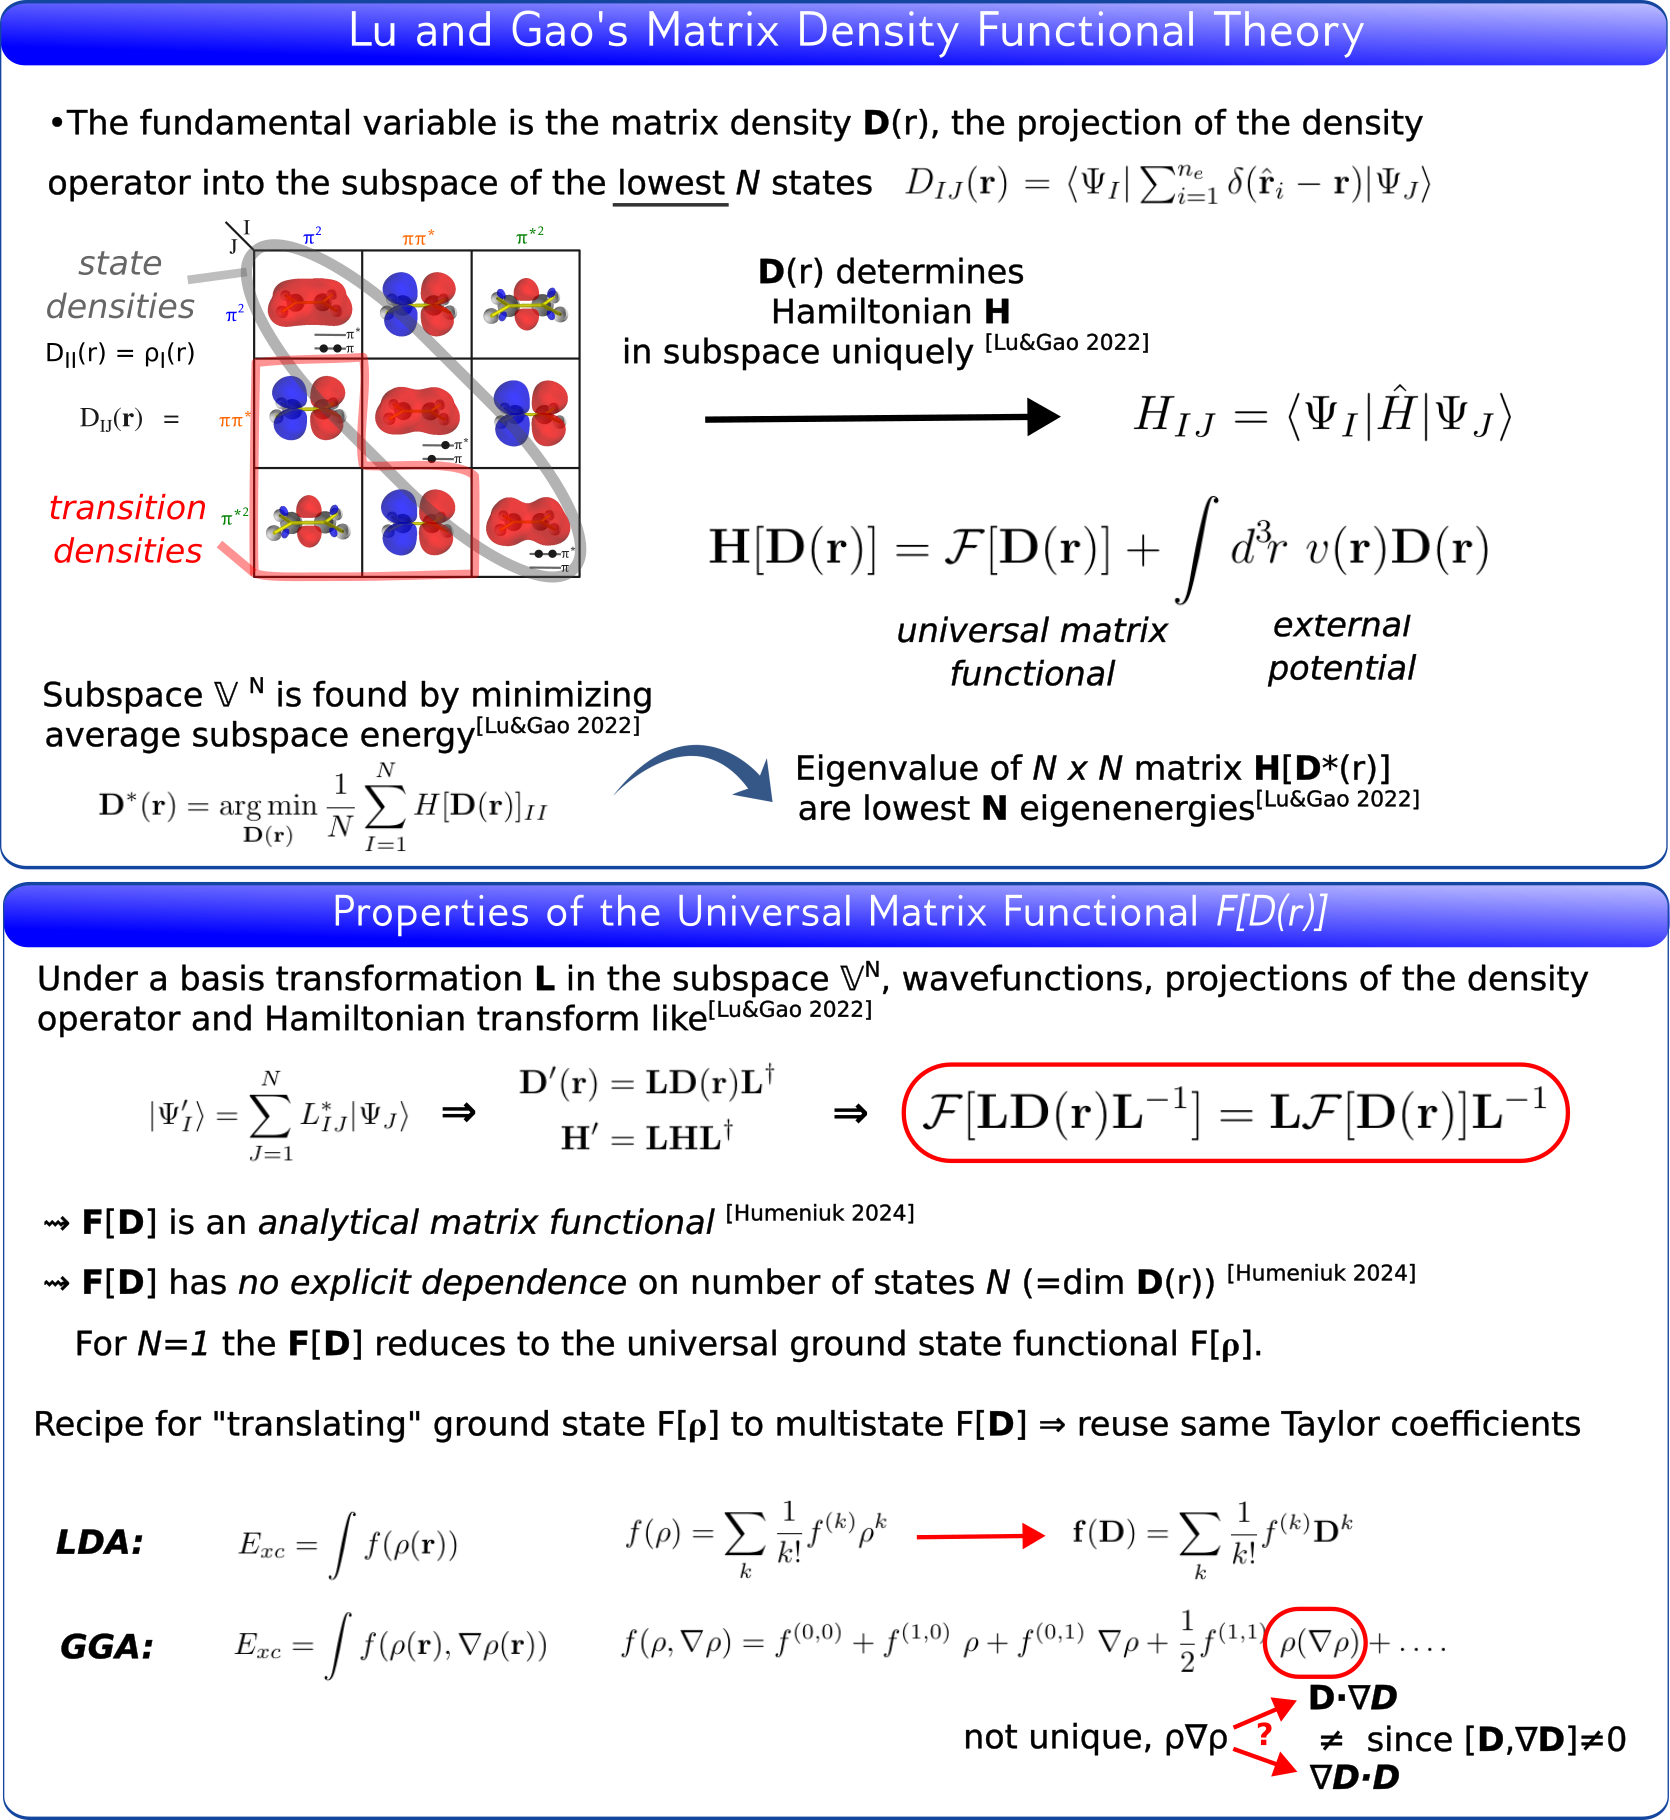
\includegraphics[width=1.0\linewidth]{figures/basic_ideas_of_msdft.png}
    \caption{\label{fig:basic_ideas_of_msdft} Basic ideas of multistate DFT.}
\end{figure}

\section{Research Plan and Methods}

\subsection{Fundamental open questions \label{sec:fundamentals}}
\begin{enumerate}
\item The whole theory rests on the assumption that the universal matrix functional does not explicitly depend on the number of electronic states in the subspace. A plausible argument for this was given in Ref.~\cite{Humeniuk2024}, however a more rigorous proof is desirable.
\item Which conditions does a matrix function have to fulfill to ensure that it is the matrix density of a systems of Fermions? 
This is the multistate version of the N-representability problem. 
Is it possible to perform a minimization over all matrix densities without parameterizing the matrix density in terms of (non-orthogonal) Slater determinants of single particle orbitals?
\item What exact constraints on kinetic, exchange and correlation functionals can be leveraged to limit the ambiguity due to non-commuting matrices?
\item What is the relationship between multistate DFT and other excited state theories such as ensemble DFT and time-dependent DFT?
\end{enumerate}

\subsection{Approximate multistate density functionals \label{sec:approximation}}
For practical MSDFT calculations one has to approximate the universal matrix functional $\m{\mathcal{F}}[\m{D}(\vec{r})]$.
Since a multistate functional reduces to the ground state functional in the limit of a single state,
many techniques for designing ground state functional approximations carry over to the multistate case.
Even with a simple local density approximation (LDA) both diagonal and off-diagonal elements of the electron-repulsion part of the Hamiltonian
can be predicted with surprising accuracy \cite{Humeniuk2024}. 
In analogy with ground state DFT one can climb the rungs of Jacob's ladder (employing local, semilocal and generalized gradient approximations (GGA))
to come closer to the true functional. However, there is a fundamental difference that complicates things when the functional depends on, let's say, the density and its gradient or the total density and the spin polarization: Since $\m{D}(\vec{r})$ is
a matrix and matrix-matrix multiplication is not commutative, the order of factors matter. For instance, since $\m{D}(\vec{r})$ and its
gradient $\nabla \m{D}(\vec{r})$ do not commute, there is an infinite number of different GGA-like functionals, which all reduce to
the corresponding ground state functional for a one-dimensional $\m{D}(\vec{r}) = \rho(\vec{r})$ and differ only by the order of the factors in the multivariate Taylor series. Exact conditions have to be found
in order to constrain this ambiguity. An obvious condition is that the resulting Hamiltonian matrix should be Hermitian, but more elaborate conditions can be found: In Ref. \cite{Humeniuk2024} a von-Weizs\"{a}cker-like kinetic energy functional is constrained by the requirement that it should give the exact kinetic energy matrix for a single electron. However, these conditions are not sufficient to determine
the functional uniquely and more fundamental work is needed to go beyond the LDA. In particular, it is important to know which exact conditions
of ground state DFT remain valid in MSDFT.

While exact conditions will be an essential guide in the design of multistate functionals,
some free parameters (such as the precise functional form of the enhancement factor in a GGA functional)
could be chosen in an optimal fashion by machine learning.
Since the multistate functional is analytical and independent of the number of electronic states,
training data from calculations of ground and excited state calculations can be combined to fit a single functional.
Especially the kinetic functional, for which there is no good (semilocal) approximations, could benefit from machine learning.

\subsection{Implementation of efficient computational method \label{sec:implementation}}
The proposed theory potentially lends itself to a very efficient linear-scaling implementation that allows to describe
electronic excitations in complex systems. The subspace of the lowest few states can be found by direct minimization of the subspace energy as a function of the matrix density (see Fig.~\ref{fig:basic_ideas_of_msdft}). If the matrix density is
updated using gradient descent, $\m{D}(\vec{r})_{n+1} = \m{D}(\vec{r})_{n} - \gamma \frac{d E_{\text{MS}}[\m{D}(\vec{r}')]}{d \m{D}(\vec{r})}$,
the time per optimization step scales linearly in the number of parameters.
The number of parameters for describing the matrix density is determined by the number of spatial grid points
and not the number of electrons, and relatively coarse grids could be employed in combination with pseudo potentials.
In particular no large scale eigenvalue problem has to be solved.
With semilocal exchange-correlation and kinetic energy functionals the bottleneck would be the solution of
the Poisson equation.

However, before this best-case scenario can be realized, at least two fundamental obstacles have to be overcome:

\textbf{(1) Representation of matrix density:}
One has to ensure that the $\m{D}(\vec{r})$'s visited during the optimization all correspond to matrices of state and transition densities of a Fermionic system. However, one has to be careful, as state and transition densities cannot be varied independently of each other.
This issue can be avoided by parameterizing the matrix density in terms of
a minimal number of orthogonal or non-orthogonal Slater determinants as suggested in \cite{Lu2022fundamental}. With this parameterization the scaling would be similar to CASSCF with a small active space, but linear scaling cannot be achieved easily. An orbital-free representation of the matrix density, on the other hand, would make the computational cost independent of the number of electrons in the system.

For the ground state, the square root of the density, $\psi(r) = \rho(r)^{1/2}$, can be interpreted
as a wavefunction that satisfies a Schr\"{o}dinger-like equation \cite{Levy1988exact}.
Like a single-electron orbital, the wavefunction $\psi(r)$ depends only on a single coordinate $r$,
but integrates to the total electron density. Since it has the form of an orbital, but hosts
many electrons, it is called a "collective orbital" \cite{Mi2023orbital}.
It can also be written as $\psi(r) = n \phi(r)$, where $n$ is the number of electrons
and $\phi(r)$ is normalized to $\int \phi(r)^2 d^3\!r = 1$.
This concept can be extended to multiple electronic states $N$. At each point in space $\vec{r}$, the matrix density $\m{D}(\vec{r})$ can be diagonalized giving $N$ eigenvalues $\lambda_{A}(\vec{r})$ and orthonormal eigenvectors $\tilde{\phi}_{I,A}(\vec{r})$.
We can define the (not necessarily integer) number of electrons in the "eigendensity" $\lambda_A(\vec{r})$ as
\begin{equation}
n_A = \frac{1}{N} \int \lambda_A(\vec{r}) d^3\!r.
\end{equation}
and a new set of "collective orbitals" for the eigendensity $A$,
\begin{equation}
\phi_{I,A}(\vec{r}) = \sqrt{\frac{\lambda_A(\vec{r})}{n_A}} \tilde{\phi}_{I,A}(\vec{r}),
\end{equation}
so that the matrix density can be represented as
\begin{equation}
D_{IJ}(\vec{r}) = \sum_{A=1}^{N} n_A \phi_{I,A}(\vec{r}) \phi_{J,A}(\vec{r}).
\end{equation}
The sets of collective orbitals $\phi_{I,A}(\vec{r})$ and electron occupations $n_A$ can used as independent
variational parameters of the matrix density.

Note that for a one-electron system, the matrix density is just the outer product of the wavefunctions,
\begin{equation}
D^{\text{1e}}_{IJ}(\vec{r}) = \phi^{\text{1e}}_{I}(\vec{r}) \phi^{\text{1e}}_{J}(\vec{r}),
\end{equation}
so that only a single set of collective orbitals is needed.
However, in the general many-electron case, all electron numbers $n_A$ may be non-zero,
and one needs $N$ sets of $N$ collective orbitals to describe the matrix density.

The concept of collective orbitals might also be interesting as a tool for analysing and visualizing electronic states.
Unfortunately, even if the multistate matrix density is known, computing collective orbitals that are continuous functions of positions
turns out to be more difficult than one might think. The reason is that eigenvectors of the matrix density are not uniquely defined,
since there is the freedom to choose their orientation (sign) or mix them in case of degenerate eigenvalues.

% Eigenvectors are not uniquely defined if there are degenerate eigenvalues
% Difficult to define eigenfunctions and eigenvalues that are continuous functions of position.

\textbf{(2) Orbital-free kinetic functional:}
For a linear-scaling, orbital-free implementation a (semilocal) kinetic energy functional of comparable accuracy as the exchange-correlation functional is required, which so far has been elusive. While hand-crafted kinetic functionals cannot compete with Kohn-Sham DFT in terms of accuracy, machine-learned orbital-free kinetic energy functionals have recently closed this gap. \cite{Zhang2024overcoming} Machine-learning (ML) is ideally suited to finding approximate kinetic functionals, since synthetic training data can be generated easily as the kinetic energy density can be calculated exactly from an approximate wavefunction. Building physical symmetries such as equivariance under translation and rotation into the ML architecture has proven crucial to obtain transferable and reliable density functionals. \cite{Gong2023general} 
In the case of multistate functionals an additional equivariance operation in the space of electronic states comes into play:
A neural network (NN) for approximating analytical matrix functionals has to satisfy
\begin{equation}
\mathcal{F}_{NN}[\m{L} \m{D}(\vec{r}) \m{L}^{-1}] = \m{L} \mathcal{F}_{NN}[\m{D}(\vec{r})] \m{L}^{-1} \label{eqn:transformation_property}
\end{equation}
for any basis transformation $\m{L} \in O(N)$. For equivariant ML models which preserve rotational symmetry ($SO(3)$) special libraries exist (such as e3nn \cite{Geiger2022e3nn}) that implement equivariant building blocks (linear layers and non-linear activation functions)
for assembling arbitrarily complex networks.
No such libraries are available so far for desining ML models that have the transformation property of Eqn.~\ref{eqn:transformation_property} baked into them. Desining such a library would be an important step in this project. In principle, there is a simple recipe to incorporate the transformation property: To turn a non-linear function $f(x)$ into an analytic matrix function $F(\m{D})$, one has to diagonalize $\m{D}$, apply the nonlinearity to the eigenvalues and transform back again. However, diagonalization scales unfavourably with the matrix dimension (number of electronic states) and better ideas are needed.

It is important to note that a neural network satisfying the transformation property \ref{eqn:transformation_property} can accept matrix densities with any number of states, since it approximates an analytic matrix functional. Therefore a functional that learns the interactions between state densities and transition densities can generalize to an arbitrary number of electronic states. It is thus possible to train on small molecules with few electronic states and generalize to large molecules or solids with many electronic states.
%Preliminary experiments by the author to train the enhancement factor over the Thomas-Fermi kinetic energy using a feed-forward neural network has shown that analytical matrix functionals is feasible.

% orbital-free DFT \cite{Zhang2024overcoming}
% MACHINE LEARNED KINETIC FUNCTIONAL, equivariant machine learning, compose neural network for enhancement factor from layers that preserve transformation properties of the matrix density.
% Training data can be generated easily, since the kinetic energy density can be calculated exactly from wavefunctions.
% Semilocal functional form, which depends only on the matrix density and its gradient and Laplacian probably not enough
% Train on small molecules with few electronic states and generalize to  large molecules with arbitrary number of states.
% Neural network for modeling analytical matrix functionals.
% The transformation property F[L^-1 D L] = L^-1 F[D] L is a form of equivariance.
% Equivariant ML models, which preserve rotational symmetry have become very popular recently \cite{Gong2023general}.
% A functional that learns the interactions between state densities and transition densities can generalize to an arbitrary number of electronic states.
% To incorporate the property, one has to diagonalize D, apply the nonlinearity to the eigenvalues and transform back again. This scales very badly with the number of states. Need better approximations.

\vspace{10px}
%While these fundamental questions are very hard nuts to crack,
Multistate DFT also opens a simple way to treat large systems, at least approximately. Since it is a variational theory, a large system can be described by a trial matrix density, which depends only on a few parameters that are optimized. For instance, the matrix density of a large molecular aggregate could be built up from the monomer (transition) densities with some undetermined weights.

The concrete architecture of the computer code for MSDFT calculations will hopefully crystallize during the course of the investigation.

\section{Research Environment}
This work requires a quiet environment, time to think, access to scientific literature, pen and paper and a computer.
Some of the fundamental questions are very hard nuts to crack. Therefore the possibility to collaborate and exchange ideas with other scientist working on DFT-related problems would be very helpful.
At a later stage access to a high-performance computer cluster (ideally with some GPU nodes) and licenses for common quantum-chemistry software packages would be advantageous. 

\bibliographystyle{unsrt}
\bibliography{references}

\end{document}
